\documentclass[11pt]{article}

\usepackage[T1]{fontenc}
\usepackage[margin=0.75in]{geometry}
\usepackage{amsmath,amssymb}
\usepackage{booktabs}
\usepackage{graphicx}
\usepackage{microtype}
\usepackage{caption}
\usepackage{placeins}
\usepackage{float}
\usepackage{xcolor}
\usepackage{enumitem}
\usepackage{needspace}
\usepackage{xurl}
\usepackage{hyperref}
\usepackage[backend=biber,style=numeric-comp,sorting=none,maxbibnames=3,giveninits=true,url=false]{biblatex}
\addbibresource{references.bib}
\renewcommand*{\bibfont}{\scriptsize}

\graphicspath{{figures/}}
\hypersetup{pdftitle={Longitudinal Gaps and Readout Connectivity in a Pilot Generative Model of Zero-Degree Calorimeter Showers},pdfauthor={Julian Juan},pdfsubject={Pilot calorimeter-shower model and validation-sample diagnostics},colorlinks=true,linkcolor=blue!45!black,citecolor=blue!45!black,urlcolor=blue!55!black}
\captionsetup{font=small,labelfont=bf}
\setlist{nosep,leftmargin=*}
\newcommand{\GeV}{\,\mathrm{GeV}}
\newcommand{\MeV}{\,\mathrm{MeV}}
\newcommand{\Kinc}{K_{\mathrm{inc}}}
\newcommand{\Y}{\mathbf{Y}}

\title{Longitudinal Gaps and Readout Connectivity in a Pilot\\Generative Model of Zero-Degree Calorimeter Showers}
\author{Julian Juan\\[3pt]\small\href{mailto:juliansjuan08@gmail.com}{juliansjuan08@gmail.com}}
\date{September 2026}

\begin{document}
\maketitle

\begin{abstract}
A generative calorimeter surrogate can reproduce the mean energy response and the mean occupancy of the reference simulation and still organise its showers differently in space. We quantify this for a hierarchical generator, built from discrete sampling stages and two conditional flow-matching models, for single neutrons in a simulated Zero-Degree Calorimeter of the ePIC experiment with 65 longitudinal layers and 6,790 readout channels. It is trained on 26,624 Geant4 showers and compared with Geant4 at 10,000 matched incident neutrons of 50--250\,GeV kinetic energy, using raw energy deposits with no readout threshold. The mean total deposit agrees to 1.0\% and the mean number of active layers to 0.25 layers. The spatial structure does not agree. Among nonempty showers, the last active layer of a generated shower lies 4.42 layers deeper on average, its occupied depth range contains 3.95 more empty layers, and 93.5\% of generated showers have at least one empty layer inside that range, against 52.4\% for Geant4. The mean number of connected components on the readout graph rises from 23.42 to 59.39. An algebraic bound shows that the extra empty layers can account for at most 5.52 of these 35.97 additional components; at least 30.45 (84.6\%) arise within runs of contiguous active layers. A classifier trained on shower-shape summaries separates the two samples with an AUROC of 0.775. The results describe one training run on 4\% of the available training events; their sensitivity to a readout threshold has not yet been measured, and no detector-performance claim is made.
\end{abstract}

\section{Introduction}

At the Electron-Ion Collider, neutrons and photons emitted within a few milliradians of the hadron beam will be measured by a zero-degree calorimeter (ZDC) about 35\,m downstream of the interaction point. The design study for a SiPM-on-tile ZDC reconstructs neutron energy and angle from individual hits with graph neural networks, against requirements of $50\%/\sqrt{E}$ in energy and $3\,\mathrm{mrad}/\sqrt{E}$ in angle~\cite{epiczdc}. Reconstruction of this kind uses where the hits are, not only how much energy they sum to. A fast simulation meant to replace detailed Geant4 transport~\cite{geant4} for such a detector therefore has to reproduce the spatial pattern of deposits.

Generative calorimeter models have used normalizing flows, diffusion, and conditional flow matching on regular grids, point clouds, and graphs~\cite{caloflow,calodiffusion,calograph,caloclouds2,calodream}. The CaloChallenge compares them on energy, shower-shape, classifier, and computing-cost observables~\cite{calochallenge,kansalmetrics}. For the ALICE ZDC, variational autoencoders, adversarial models, diffusion, flow matching, and mixtures of generative experts have been studied~\cite{dubinskizdc,kitazdc,fasterzdc,expertsim,wojnar2025}; recent flow models address output variability~\cite{majerziaf} and the co-activation of neighbouring channels~\cite{majerz2026}. Those detectors, targets and representations differ from ours, so their quoted fidelities are context and not baselines.

This paper studies one hierarchical generator for neutron showers in an ePIC ZDC simulation and asks a narrow question: \emph{if the generated and reference samples agree in mean deposited energy and mean occupancy, do they also agree in longitudinal and graph structure?} For the model studied here the answer is no. The paper makes three contributions.
\begin{enumerate}
 \item A complete specification of the generator, from the incident four-vector to 6,790 channel energies (Sec.~\ref{sec:model}), so that each observable can be traced to the stage that produces it.
 \item Two structural observables---the number of empty layers inside the occupied depth range and the number of connected components on the readout graph---together with an algebraic bound that separates longitudinal splitting from fragmentation within contiguous layers using sample means alone (Sec.~\ref{sec:diagnostics}).
 \item A comparison with Geant4 at 10,000 matched incident neutrons (Sec.~\ref{sec:results}), a candidate mechanism for the discrepancy, and the measurements that would confirm or exclude it (Sec.~\ref{sec:discussion}).
\end{enumerate}

\paragraph{Scope.} The results are for a single training run of a single architecture, trained on 4.35\% of the available training events, and for raw deposits with no readout threshold or digitisation. The evaluation sample was reused during model development and is not a blind test. The analysis uses the summary statistics written by the evaluation run (means, mean layer profiles, selected distances and bootstrap intervals), not per-event arrays; quantities that need per-event information, such as distributions of the structural observables or their dependence on a threshold, are listed as follow-up measurements in Sec.~\ref{sec:discussion}. We do not claim detector-level fidelity, a speed-up, or an advantage over other architectures.

\section{Detector simulation and data}
\label{sec:data}

\subsection{Detector and readout channels}

The data are Geant4~\cite{geant4} showers of single neutrons in an ePIC ZDC geometry. The geometry stored with the sample has 65 longitudinal layers (Fig.~\ref{fig:geometry}). Layer~0 is an electromagnetic section (ECAL) of 400 channels in a $20\times20$ array with 30.3\,mm pitch. Layers 1--64 form the hadronic section (HCAL), with 100 channels per layer in layers 1--63 and 90 in layer~64, a layer pitch of 24.9\,mm, and 1.57\,m between its first and last layers. Neighbouring HCAL channels within a layer are typically 54\,mm apart. The ECAL lies 35.7\,m from the coordinate origin and the detector axis points at $-25.0$\,mrad in the horizontal plane, consistent with a frame centred on the interaction point and the 25\,mrad beam-crossing angle of the EIC.

These dimensions match the SiPM-on-tile design of Refs.~\cite{epiczdc,hexplit}: steel absorber with 3\,mm hexagonal scintillator tiles of 25\,cm$^2$ in a staggered arrangement, an envelope of $60\times60\times162$\,cm$^3$, and a depth of about seven nuclear interaction lengths at $z\approx35$\,m. We could not, however, check the sample against a tagged production geometry, and its Geant4 version, physics list, production cuts and readout time window were not recorded with it. Layer indices should therefore be read as indices; we do not convert them to interaction lengths.

A \emph{channel} in this paper is one distinct cell identifier in the stored sample. For 2,400 of the 6,390 HCAL identifiers, hits are recorded at two to four distinct positions (1,950, 444 and 6 identifiers, respectively); such a channel is placed at the unweighted centroid of its positions. Whether this reflects intended grouping of tiles or an artefact of the identifier encoding cannot be decided without the production identifier map. Channel-level statements below therefore refer to stored identifiers, not to verified electronics channels.

\begin{figure}[!htbp]
 \centering
 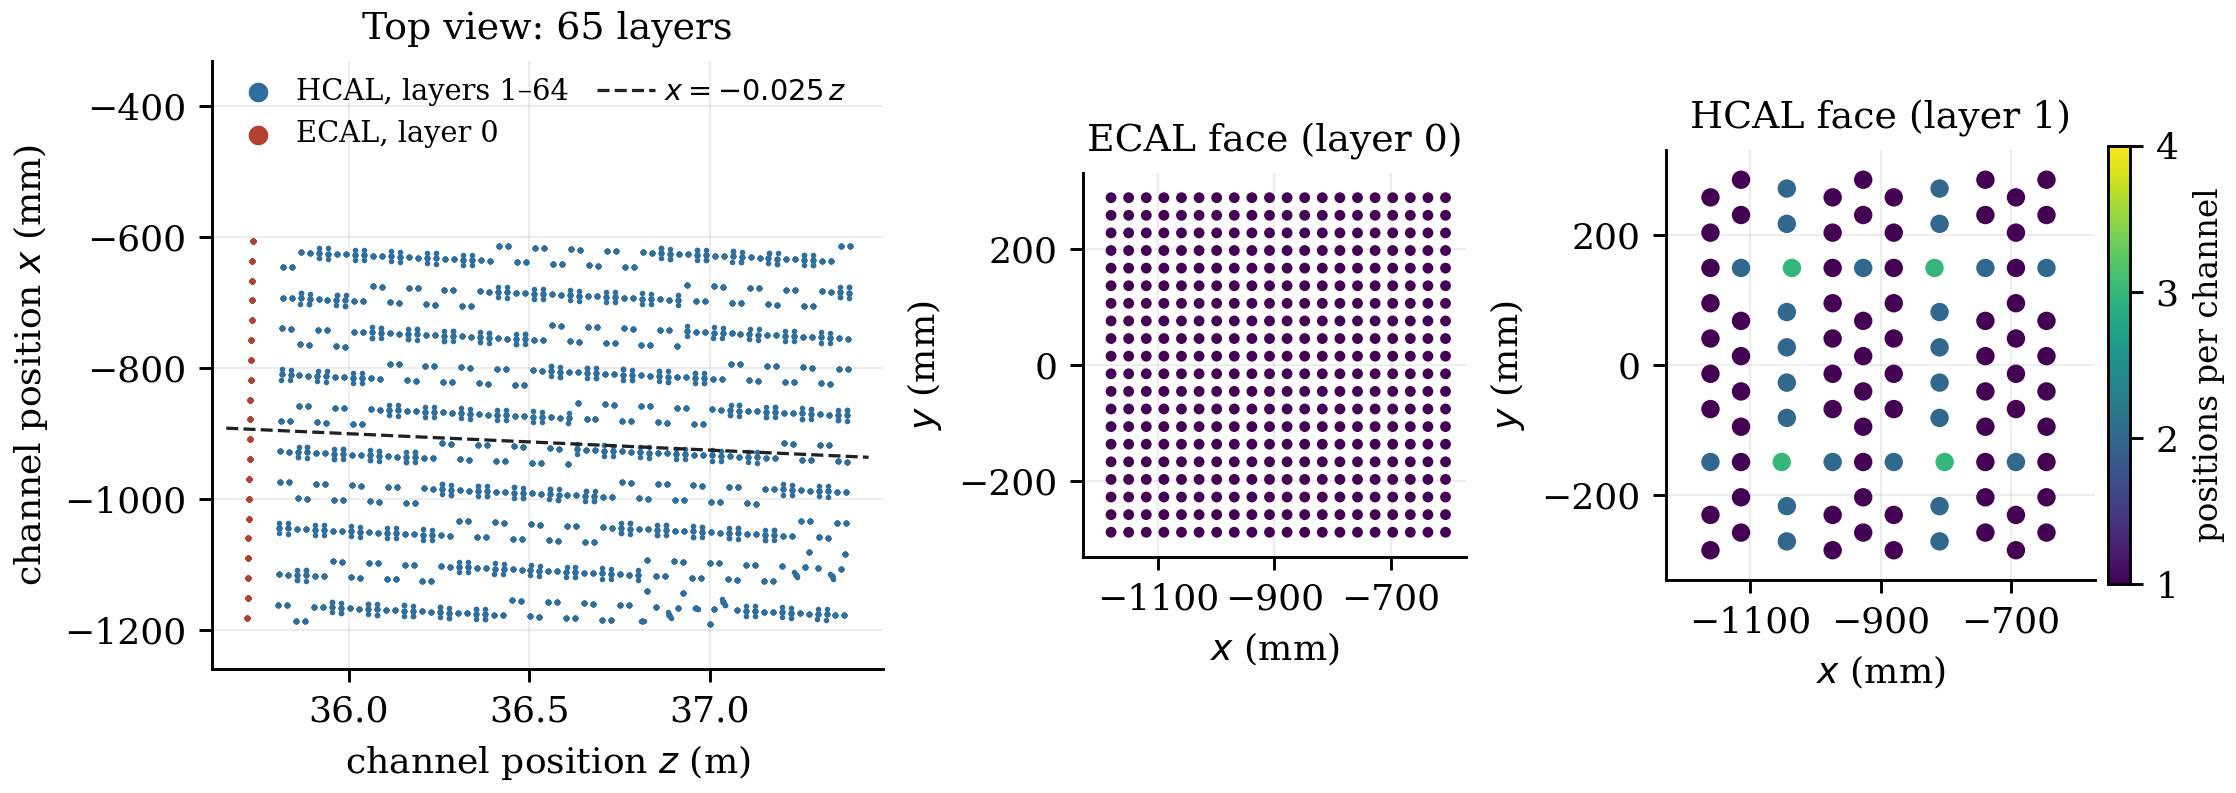
\includegraphics[width=\linewidth]{detector_layout.png}
 \caption{Channel positions stored with the sample. Left: all 6,790 channels projected on the horizontal plane; the single ECAL layer precedes 64 HCAL layers, and the dashed line marks a direction of $-25$\,mrad from the origin (axes are not to the same scale). Centre and right: the ECAL face and the first HCAL layer. Colour gives the number of distinct hit positions sharing one channel identifier; such channels are placed at the centroid of their positions. This figure defines the nodes of the graph used by both the generator and the connectivity observable.}
 \label{fig:geometry}
\end{figure}

\subsection{Target and conditioning}

The target $\Y\in\mathbb R_{\geq0}^{6790}$ is the energy deposited in each channel, summed over all simulation hits with the same identifier. No digitisation, energy threshold or additional time cut is applied. The event total $T=\sum_i Y_i$ is the summed deposit recorded by the readout, not the incident energy: its mean is 4.3\,GeV for a mean incident kinetic energy of 150\,GeV. The ECAL and HCAL deposits are added without calibration weights. Their means are comparable (Sec.~\ref{sec:results}) although the ECAL is a single layer, and the event-to-event spread of $T$ is as large as its mean (Appendix~\ref{app:additional}); both features are what one expects if a homogeneous ECAL precedes a sampling HCAL, but we have not verified the ECAL material. An event with $T=0$ is called an \emph{empty shower}.

Each event is conditioned on the incident-neutron four-vector $p^\mu=(E,p_x,p_y,p_z)$ in GeV, from which five network inputs are formed:
\begin{equation}
 c=\left(\log(1+\Kinc/100\GeV),\,u_x,\,u_y,\,u_z,\,\log(E/\GeV)\right),
 \qquad \mathbf u=\frac{\mathbf p}{\max(\lVert\mathbf p\rVert,10^{-12}\GeV)},
 \label{eq:condition}
\end{equation}
where $\Kinc=\max(E-m_n,0)$ is the kinetic energy and $m_n=0.93956542052\GeV$. The two energy inputs carry the same information for $E\geq m_n$; both were present when the model was trained, so both are listed. The denominator floor only protects against division by zero. The condition contains no impact position: whether the direction fixes the impact point depends on the production vertex, which we did not verify (Sec.~\ref{sec:limitations}).

\subsection{Readout graph}

Both the generator and the connectivity observable use one fixed graph on the 6,790 channels. Each channel is linked to its eight nearest neighbours in the same layer. Each channel in layers 0--63 is also linked to its four nearest channels in the next layer, and every such longitudinal link is stored in both directions. This gives $8\times6790=54{,}320$ lateral and $2\times4\times(400+63\times100)=53{,}600$ longitudinal directed edges, 107,920 in total. Adjacency is defined by distances between channel positions; it is a property of this representation and has not been compared with a physical-neighbour map of the detector.

\subsection{Training and evaluation samples}

The full sample contains 764,940 showers with kinetic energies of 0--300\,GeV. A deterministic hash of the event identifier assigns 612,482 events to training, 76,158 to validation and 76,300 to test. The model analysed here is a pilot: it was trained on 26,624 training events (4.35\% of the training partition), with 6,656 validation events used to select the checkpoint.

\Needspace{6\baselineskip}
The evaluation uses 10,000 incident neutrons drawn from the validation partition with $50\leq\Kinc\leq250\GeV$, spread approximately uniformly in energy (1,182 to 1,310 events in each 25\,GeV bin). For each four-vector we compare the stored Geant4 shower with one shower drawn independently from the generator. The two showers of a pair share the incident condition and nothing else. This evaluation sample was inspected repeatedly while the model was developed, so it is not a blind test, and its overlap with the 6,656 selection events was not recorded. No event from the test partition is used.

\section{Generator and training}
\label{sec:model}

The generator builds a shower in three levels (Fig.~\ref{fig:architecture} and Table~\ref{tab:stages}). It first decides how much energy the readout records ($T$), then where along the detector that energy appears ($F,\mathbf A,\mathbf B$), and finally which channels in each layer are hit and how the layer energy is shared among them ($\mathbf K,\mathbf S,\Y$). Sampling the number of hits before their positions follows point-cloud models~\cite{caloclouds2,calopointflow}. The stages model the outcome of a shower; they do not simulate individual interactions.

The model has 2,082,507 trainable parameters. A two-block residual multilayer perceptron maps the five inputs of Eq.~\eqref{eq:condition} to a 128-component condition vector $h_c$ that every later stage receives. The discrete stages are sampled from learned probabilities; the two continuous stages are conditional flow-matching models that start from independent Gaussian noise. No latent variable is shared across stages: all dependence between stages is carried by the quantities sampled upstream. The random draws represent shower-to-shower fluctuations at fixed incident condition, not electronics noise.

Throughout, $\ell=0,\ldots,64$ indexes layers, $i$ indexes the channels of layer $\ell$, and $Y_{\ell i}$ is a channel deposit. A channel is \emph{active} if $Y_{\ell i}>0$. A layer is active if its energy $B_\ell=\sum_iY_{\ell i}$ is positive. The event total is $T=\sum_\ell B_\ell$. A star marks a quantity taken from a Geant4 shower.

\begin{figure}[!htbp]
 \centering
 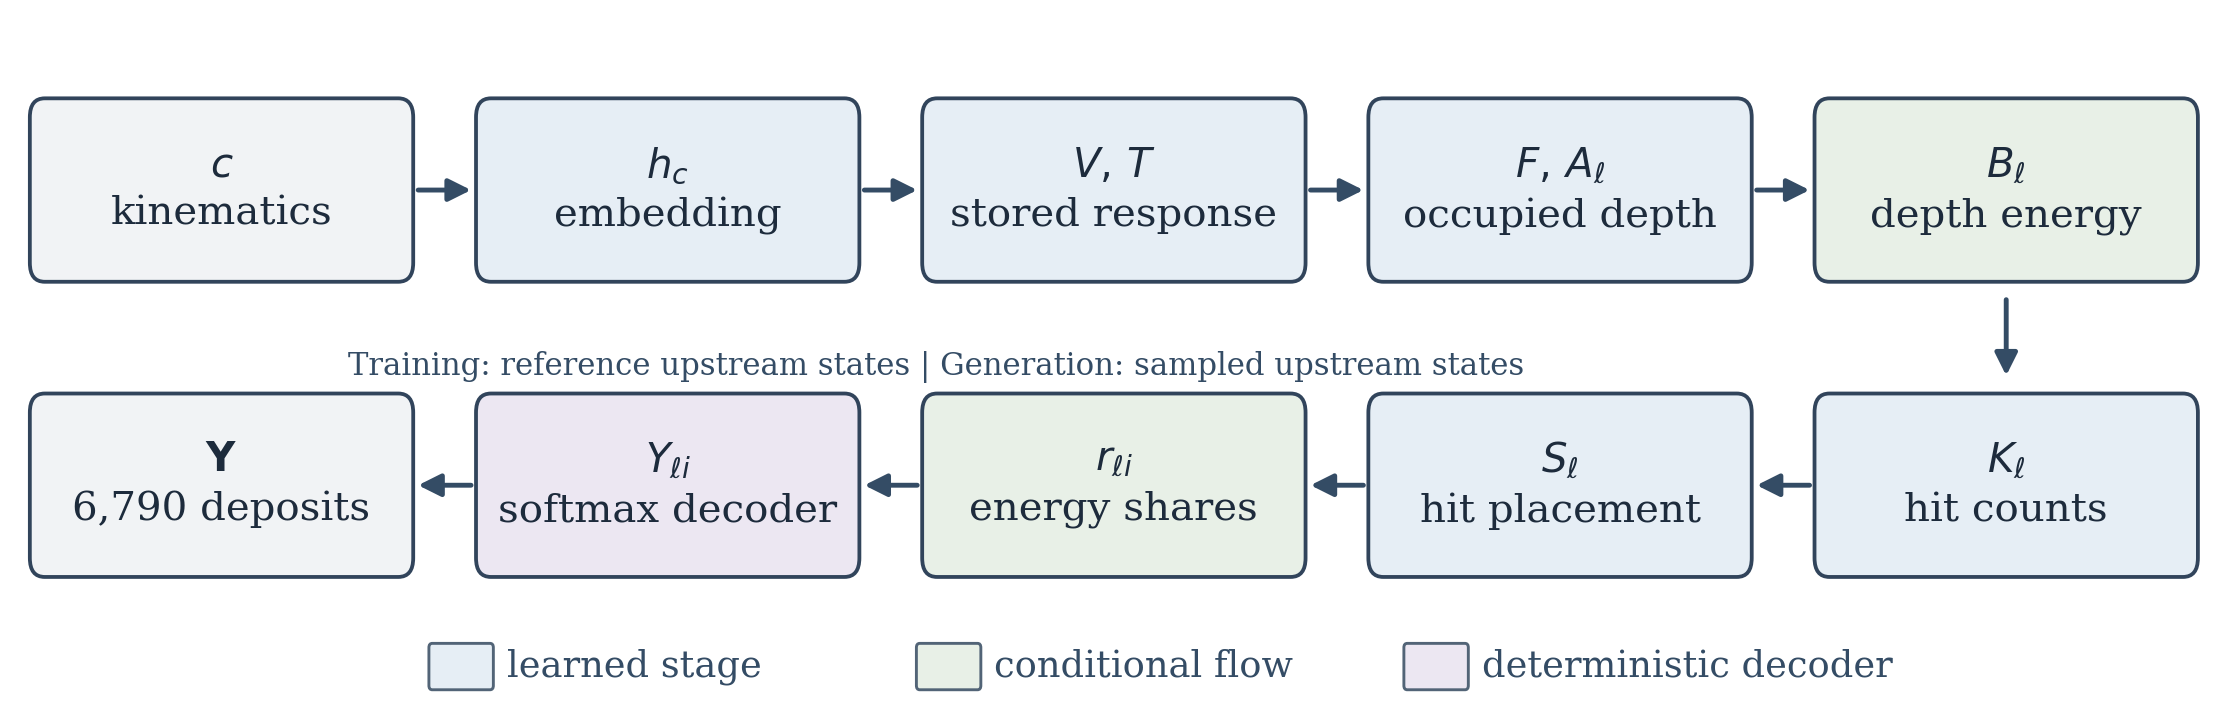
\includegraphics[width=\linewidth]{generator_schematic.png}
 \caption{Generation order: top row left to right, then bottom row right to left. Blue stages are sampled from learned discrete or mixture distributions, green stages are conditional flows, and the purple stage is a deterministic softmax. Arrows show the order of sampling, not every conditioning link. During training each stage receives the upstream quantities of the Geant4 shower; during generation it receives the sampled ones.}
 \label{fig:architecture}
\end{figure}

\begin{table}[H]
\centering
\caption{Stages of the generator in sampling order. Every stage is also conditioned on $h_c$. The last column names the argument of the corresponding loss term in Eq.~\eqref{eq:joint_loss}; channel selection has two terms.}
\label{tab:stages}
\small
\begin{tabular}{@{}llllc@{}}
\toprule
Stage & Output & Conditioned on & Model & Loss \\
\midrule
Response & visibility $V$, total $T$ & --- & Bernoulli; Gaussian mixture & $V$, $T$ \\
First layer & $F$ & $T$ & categorical over 65 layers & $F$ \\
Layer activity & $A_\ell$ for $\ell>F$ & $T$, $F$ & independent Bernoulli per layer & $\mathbf A$ \\
Layer energies & $B_\ell$ & $T$, $\mathbf A$ & flow, 2-layer transformer, 8 steps & $B$ \\
Channel counts & $K_\ell$ & $B_\ell$, $A_\ell$ & categorical per layer & $\mathbf K$ \\
Channel selection & $S_\ell$ & $\mathbf B$, $\mathbf K$ & graph-network scores; Gumbel top-$K$ & $\mathbf S$ \\
Channel energies & $Y_{\ell i}$ & $\mathbf B$, $\mathbf K$, $\mathbf S$ & flow, graph network, 8 steps; softmax & $Y$ \\
\bottomrule
\end{tabular}
\end{table}

\subsection{Total deposit and longitudinal allocation}

\paragraph{Total deposit.} The response stage is a hurdle model: it first decides whether the readout records any energy, then draws how much. We call an event \emph{visible} if $T>0$. A Bernoulli head draws a provisional flag $V_0$, and a four-component Gaussian mixture describes the transformed total $q_T$. The Bernoulli logit $a_\theta$, the mixture means $\mu_m$, widths $\sigma_m>0$, and weights $\omega_m$ are functions of $h_c$; $\theta$ denotes the learned parameters and $\sigma(\cdot)$ the logistic function:
\begin{equation}
 \begin{aligned}
 \Pr(V_0=1\mid h_c)&=\sigma(a_\theta(h_c)),
 &q_T&=\log(1+T/10\GeV),\\
 p_\theta(q\mid h_c)&=\sum_{m=1}^{4}\omega_m(h_c)
 \mathcal N\!\left(q;\mu_m(h_c),\sigma_m^2(h_c)\right).
 \end{aligned}
 \label{eq:response_transform}
\end{equation}
A draw $q$ is transformed back to GeV, clipped at zero, and capped at $C(\Kinc)$:
\begin{equation}
 \begin{aligned}
 C(\Kinc)&=\min\{0.630110\max(\Kinc,1\GeV),61.2338\GeV\},\\
 T_{\mathrm{cand}}&=\min\{10\GeV\max(e^q-1,0),C(\Kinc)\},\\
 V&=V_0\,\mathbf 1_{\Kinc>0}\,\mathbf 1_{T_{\mathrm{cand}}>0},
 \qquad T=VT_{\mathrm{cand}}.
 \end{aligned}
 \label{eq:cap}
\end{equation}
The cap is a safeguard against extreme draws from the tail of the mixture. Its constants were derived from the training sample, it saturates at 61.2338\,GeV above $\Kinc\approx97.2\GeV$, and it lies far above the mean deposit of a few GeV. An event is empty either because $V_0=0$ or because a mixture draw falls at or below zero.

\paragraph{Active layers.} For a visible event the model draws the first active layer $F$ from a 65-way categorical distribution with logits $f_\theta(h_c,\log(1+T/\GeV))$, and sets all earlier layers inactive. $F$ is the first layer with a recorded deposit, which need not be the layer of the first inelastic interaction. Each later layer is then switched on or off by its own Bernoulli draw:
\begin{equation}
 p(\mathbf A\mid h_c,T,F)=\prod_{\ell>F}^{64}p(A_\ell\mid h_c,T,F,\ell),
 \qquad A_F=1.
 \label{eq:activity}
\end{equation}
The activity mask $\mathbf A$ fixes the occupied depth range and the empty layers inside it. Equation~\eqref{eq:activity} is the assumption that matters most for this paper: given $(h_c,T,F)$, the layers are switched on independently, so the model cannot represent the tendency of neighbouring layers to be active together beyond what $T$ and $F$ explain. Section~\ref{sec:interpretation} returns to this.

\paragraph{Layer energies.} A flow then distributes $T$ over the active layers, which fixes the longitudinal profile and the ECAL/HCAL split. Its training target is built from a Geant4 shower with layer energies $B_\ell^\star$, total $T^\star$ and activity $A_\ell^\star=\mathbf 1_{B_\ell^\star>0}$ as a centred log fraction,
\begin{equation}
 a_\ell^\star=\log\max\!\left(
 \frac{B_\ell^\star}{\max(T^\star,10^{-12}\GeV)},10^{-8}\right),
 \quad (x_1)_\ell=A_\ell^\star\left(
 a_\ell^\star-\frac{\sum_m A_m^\star a_m^\star}
 {\max(1,\sum_m A_m^\star)}\right).
 \label{eq:profile_target}
\end{equation}
Subtracting the mean over active layers removes the one degree of freedom that the later softmax ignores. The floors $10^{-8}$ and $10^{-12}\GeV$ keep the logarithm finite and are not detector thresholds; a layer fraction below $10^{-8}$ would be raised to that value, and how often this happens was not counted. For an empty shower the target and mask are zero.

\paragraph{Flow matching.} Both flows learn a velocity field $v_\theta$ that carries Gaussian noise $x_0$ to a target $x_1$ along the straight path $x_t=(1-t)x_0+tx_1$~\cite{flowmatching,rectifiedflow}. The flow time $t\in[0,1]$ is an interpolation parameter with no relation to detector time. With $t$ uniform on $[0,1]$ and a mask $M_{bj}\in\{0,1\}$ selecting the active coordinates $j$ of example $b$, the loss is the masked mean squared error between the predicted and the straight-path velocity,
\begin{equation}
 x_t=(1-t)x_0+t x_1,\qquad
 \mathcal L_{\mathrm{FM}}=
 \frac{\sum_{b,j}M_{bj}
 [v_\theta(x_t,t;\mathrm{ctx})_{bj}-(x_1-x_0)_{bj}]^2}
 {\max(1,\sum_{b,j}M_{bj})},
 \label{eq:cfm}
\end{equation}
where ``ctx'' stands for $h_c$ and the upstream quantities. At generation time each flow is integrated in eight steps from fresh noise:
\begin{equation}
 z_0=M\odot\varepsilon,\quad \varepsilon\sim\mathcal N(0,I),\qquad
 z_{n+1}=M\odot\left[z_n+\tfrac18
 v_\theta\!\left(z_n,\tfrac{n+1/2}{8};\mathrm{ctx}\right)\right],
 \quad n=0,\ldots,7,
 \label{eq:flow_steps}
\end{equation}
with $\odot$ the elementwise product. Each step evaluates the velocity at the current state and at the midpoint of the time interval and then resets inactive coordinates to zero. It is a first-order (Euler) step with a midpoint time, not the second-order midpoint rule.

For a visible event the final state $z_8$ of the layer flow is converted to layer energies by a softmax over the active layers,
\begin{equation}
 \pi_\ell=\frac{A_\ell e^{z_{8,\ell}}}
 {\sum_{m:A_m=1}e^{z_{8,m}}},\qquad
 B_\ell=T\pi_\ell,\qquad \sum_{\ell=0}^{64}B_\ell=T,
 \label{eq:layer_budget}
\end{equation}
so the layer energies sum to the sampled total and inactive layers receive exactly zero. The velocity network has width 128 and two transformer layers with four attention heads. Its inputs for each layer are the flow state, the activity flag, $\log(1+T/\GeV)$, $h_c$, a learned layer embedding, and a sinusoidal encoding of $t$. The attention is bidirectional: the energy assigned to a layer can depend on all other layers.

\subsection{Channel counts, channel selection, and channel energies}

\paragraph{Counts.} For each layer, a categorical head conditioned on $(h_c,B_\ell,A_\ell)$ and a learned layer embedding draws the number $K_\ell$ of active channels. A mask enforces $K_\ell=0$ for inactive layers and $1\leq K_\ell\leq N_\ell$ for active ones, where $N_\ell$ is the number of channels in the layer.

\paragraph{Selection.} A graph network assigns a score to every channel, and the $K_\ell$ channels of each layer are then drawn according to those scores. The network inputs per channel are the standardised position, the normalised layer index, ECAL/HCAL flags, $h_c$, $B_\ell$ and the requested fraction $K_\ell/N_\ell$. Three message-passing blocks of width 96 act on the edge set $\mathcal E$ of the readout graph. With $h_i^{(r)}$ the representation of channel $i$ entering block $r$ and $e_{ji}$ the five edge inputs (three coordinate differences, distance, and edge type),
\begin{equation}
 m_i^{(r)}=\sum_{j:(j,i)\in\mathcal E}
 \phi_r(h_j^{(r)},h_i^{(r)},e_{ji}),\qquad
 h_i^{(r+1)}=h_i^{(r)}+\psi_r(h_i^{(r)},m_i^{(r)}),
 \label{eq:message}
\end{equation}
where $\phi_r$ and $\psi_r$ are small multilayer perceptrons. The representations are then averaged per layer, passed through a two-layer, four-head transformer across layers, and broadcast back to the channels before the scores $s_{\ell i}$ are formed. Messages let the score of a channel depend on its neighbours. The set $S_\ell$ of active channels in layer $\ell$ (the \emph{support}) is drawn from the channels $\mathcal N_\ell$ of that layer by
\begin{equation}
 S_\ell=\left\{i\in\mathcal N_\ell:
 \operatorname{rank}_{\mathcal N_\ell}(s_{\ell i}/\tau+g_{\ell i})\leq K_\ell\right\},
 \label{eq:topk}
\end{equation}
where rank one is the largest value, $\tau=1$, and the $g_{\ell i}$ are independent Gumbel variates generated from uniform numbers clipped to $[10^{-7},1-10^{-7}]$. This Gumbel-top-$K$ rule draws $K_\ell$ distinct channels without replacement~\cite{gumbeltopk}. It fixes the number of selected channels exactly but places no constraint on their adjacency: the perturbations are independent from channel to channel, so connected support has to come from the scores alone.

\paragraph{Energies.} A second flow shares each layer energy among the selected channels. Its target for a Geant4 shower with active channels $S_\ell^\star$, $K_\ell^\star=|S_\ell^\star|>0$, is the centred log fraction of the layer energy,
\begin{equation}
 a_{\ell i}^\star=\log\max\!\left(
 \frac{Y_{\ell i}^\star}{\max(B_\ell^\star,10^{-12}\GeV)},10^{-8}\right),\qquad
 (x_1)_{\ell i}=\mathbf 1_{i\in S_\ell^\star}
 \left(a_{\ell i}^\star-\frac{1}{K_\ell^\star}
 \sum_{j\in S_\ell^\star}a_{\ell j}^\star\right),
 \label{eq:share_target}
\end{equation}
with zero target in inactive layers. It is trained with Eq.~\eqref{eq:cfm} and sampled with Eq.~\eqref{eq:flow_steps}, using $S_\ell^\star$ in training and the sampled $S_\ell$ in generation. Its velocity network has the same graph-plus-transformer structure as the selection network, with the flow state and a time encoding added to the channel inputs and unselected channels masked before and after every block. The eight steps yield logits $r_{\ell i}$, and a softmax assigns the energies:
\begin{equation}
 Y_{\ell i}=
 \begin{cases}
 B_\ell\,\dfrac{\exp r_{\ell i}}{\sum_{j\in S_\ell}\exp r_{\ell j}}, & i\in S_\ell,\\[6pt]
 0, & i\notin S_\ell.
 \end{cases}
 \label{eq:decoder}
\end{equation}

\paragraph{What the construction guarantees.} In exact arithmetic the generated shower satisfies $|S_\ell|=K_\ell$, $Y_{\ell i}\geq0$, $\sum_iY_{\ell i}=B_\ell$ and $\sum_{\ell i}Y_{\ell i}=T$. These identities say that the stages are mutually consistent; they do not express conservation of the incident energy, most of which is not recorded by the readout. They also show which stage owns which observable. Empty layers are decided by the activity stage alone. Which channels are active, and therefore the connectivity of the shower, is decided by the count and selection stages. The energy flow can move energy among selected channels but cannot add, remove or relocate a channel.

\subsection{Training and checkpoint selection}

During training every stage receives the upstream quantities of the Geant4 shower (teacher forcing). During generation it receives sampled ones, so an error in an early stage propagates to all later stages. All results in Sec.~\ref{sec:results} are therefore for complete generated showers. The training objective is a weighted sum of nine terms,
\begin{equation}
 \begin{aligned}
 \mathcal L_{\rm joint}={}&w_V\mathcal L_{\rm BCE}(V)
 +w_T\mathcal L_{\rm NLL}(T)
 +w_F\mathcal L_{\rm CE}(F)
 +w_A\mathcal L_{\rm BCE}(\mathbf A)
 +w_B\mathcal L_{\rm FM}^{B}\\
 &+w_K\mathcal L_{\rm CE}(\mathbf K)
 +w_S\mathcal L_{\rm BCE}(\mathbf S)
 +w_R\mathcal L_{\rm rank}(\mathbf S)
 +w_Y\mathcal L_{\rm FM}^{Y}.
 \end{aligned}
 \label{eq:joint_loss}
\end{equation}
Binary cross entropy (BCE) trains the visibility, layer-activity and channel-selection decisions, and categorical cross entropy (CE) the first layer and the counts. The negative log likelihood (NLL) of the total is evaluated in the variable $q_T$ of Eq.~\eqref{eq:response_transform}; expressed as a density in $T$ it acquires the Jacobian factor $1/(T+10\GeV)$. The ranking term averages $\log[1+\exp(-(s_i-s_j))]$ over sampled pairs of an active channel $i$ and an inactive channel $j$. $\mathcal L_{\rm FM}^{B}$ and $\mathcal L_{\rm FM}^{Y}$ are Eq.~\eqref{eq:cfm} for the layer and channel flows; the count term gives reduced weight to the trivial zero counts of inactive layers. The weights $w_j$ (Appendix~\ref{app:reproducibility}) were set once so that the nine terms have comparable gradient norms.

The stages were trained in sequence---response, layer profile, counts, selection, channel energies---and then jointly. The condition encoder was trained with the response stage, frozen during the other single-stage phases, and released for joint training. Optimisation used AdamW with a peak learning rate of $3\times10^{-4}$, batches of six events accumulated over four steps (effective batch size 24), gradient-norm clipping at one, and seed 20260723.

\begin{figure}[!htbp]
 \centering
 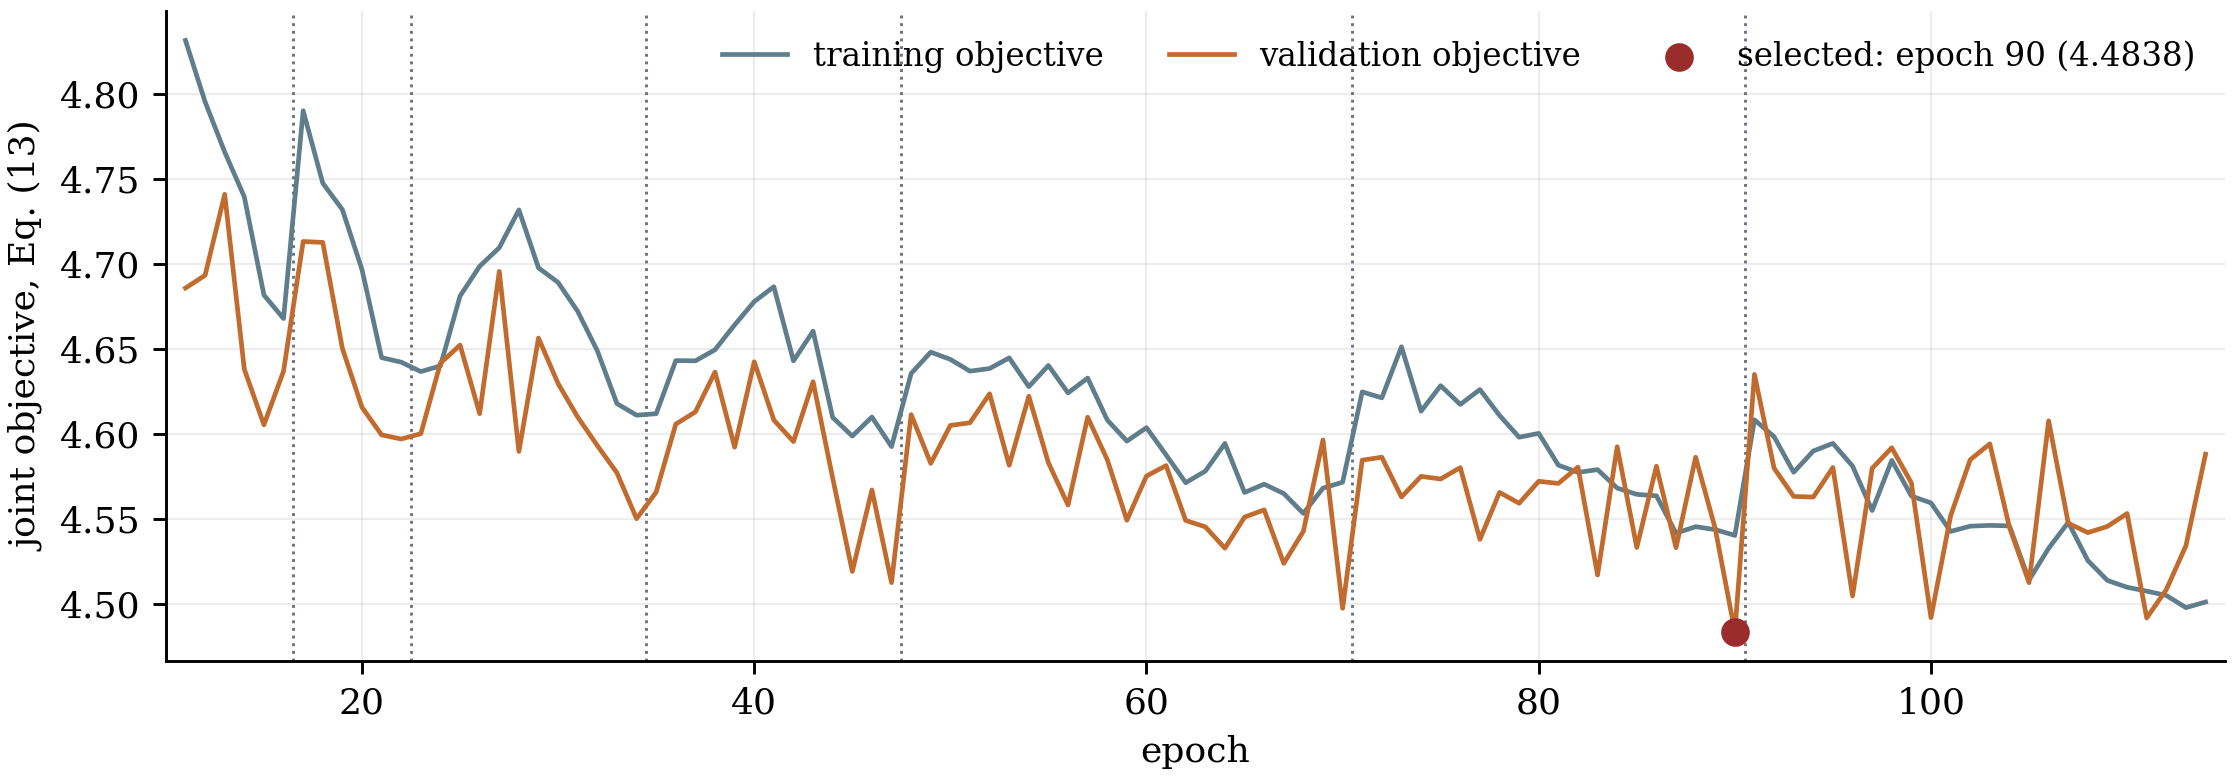
\includegraphics[width=\linewidth]{training_history.png}
 \caption{Joint objective of Eq.~\eqref{eq:joint_loss} on the training and validation subsets over the 104 available epochs of joint training. Dotted lines separate consecutive training runs, each continued from the preceding one. The objective jumps upward when a new run starts at epochs 17, 48, 71 and 91; a learning-rate restart is documented for the boundary between epochs 70 and 71. The model analysed in this paper is the one at epoch 90, the minimum of the validation curve. The training curve averages over minibatches while the weights are being updated, whereas the validation curve is evaluated after each epoch, so the two are not directly comparable in level.}
 \label{fig:training}
\end{figure}

Figure~\ref{fig:training} shows the joint objective for epochs 11--114. The checkpoint analysed here is epoch 90, which minimises the validation objective over that range. Three points bear on the interpretation of the results. First, the selection criterion is a teacher-forced loss and was fixed before the structural observables of Sec.~\ref{sec:diagnostics} were evaluated, so the chosen epoch need not be the one with the best structural agreement. Second, the validation objective is noisy: it improves by 0.20 (4\%) over one hundred epochs but changes by 0.04 on average from one epoch to the next, and epoch 90 is lower than the next-best epochs (100 and 111) by only 0.008. The selected checkpoint is one of several nearly equivalent minima. Third, after epoch 90 the training objective continues to fall while the validation objective does not, which indicates the onset of overfitting of a model with two million parameters to 26,624 training events.

\section{Observables and statistical treatment}
\label{sec:diagnostics}

We compare generated and Geant4 showers at three levels: total, ECAL and HCAL deposits; the pattern of active layers; and the pattern of active channels. Deposits are summarised over all 10,000 events, including empty showers, and in eight 25\,GeV bins of $\Kinc$. The structural observables below are defined for nonempty showers, of which there are 9,907 in the Geant4 sample and 9,858 in the generated sample. The two nonempty subsets are selected separately and do not contain exactly the same incident conditions. All structural observables call a channel or layer active if its deposit is strictly positive. Subscripts ``ref'' and ``gen'' denote the Geant4 (reference) and generated samples.

\subsection{Longitudinal activity}

For a nonempty shower let $F$ and $L$ be the first and last active layers. The occupied depth range, or \emph{span}, is $L-F+1$ layers, and the number of empty layers inside it is
\begin{equation}
 G=L-F+1-\sum_{\ell=0}^{64}A_\ell .
 \label{eq:gaps}
\end{equation}
A shower has an \emph{interior gap} if $G>0$. Figure~\ref{fig:definitions}(a) illustrates these quantities.

\begin{figure}[!htbp]
 \centering
 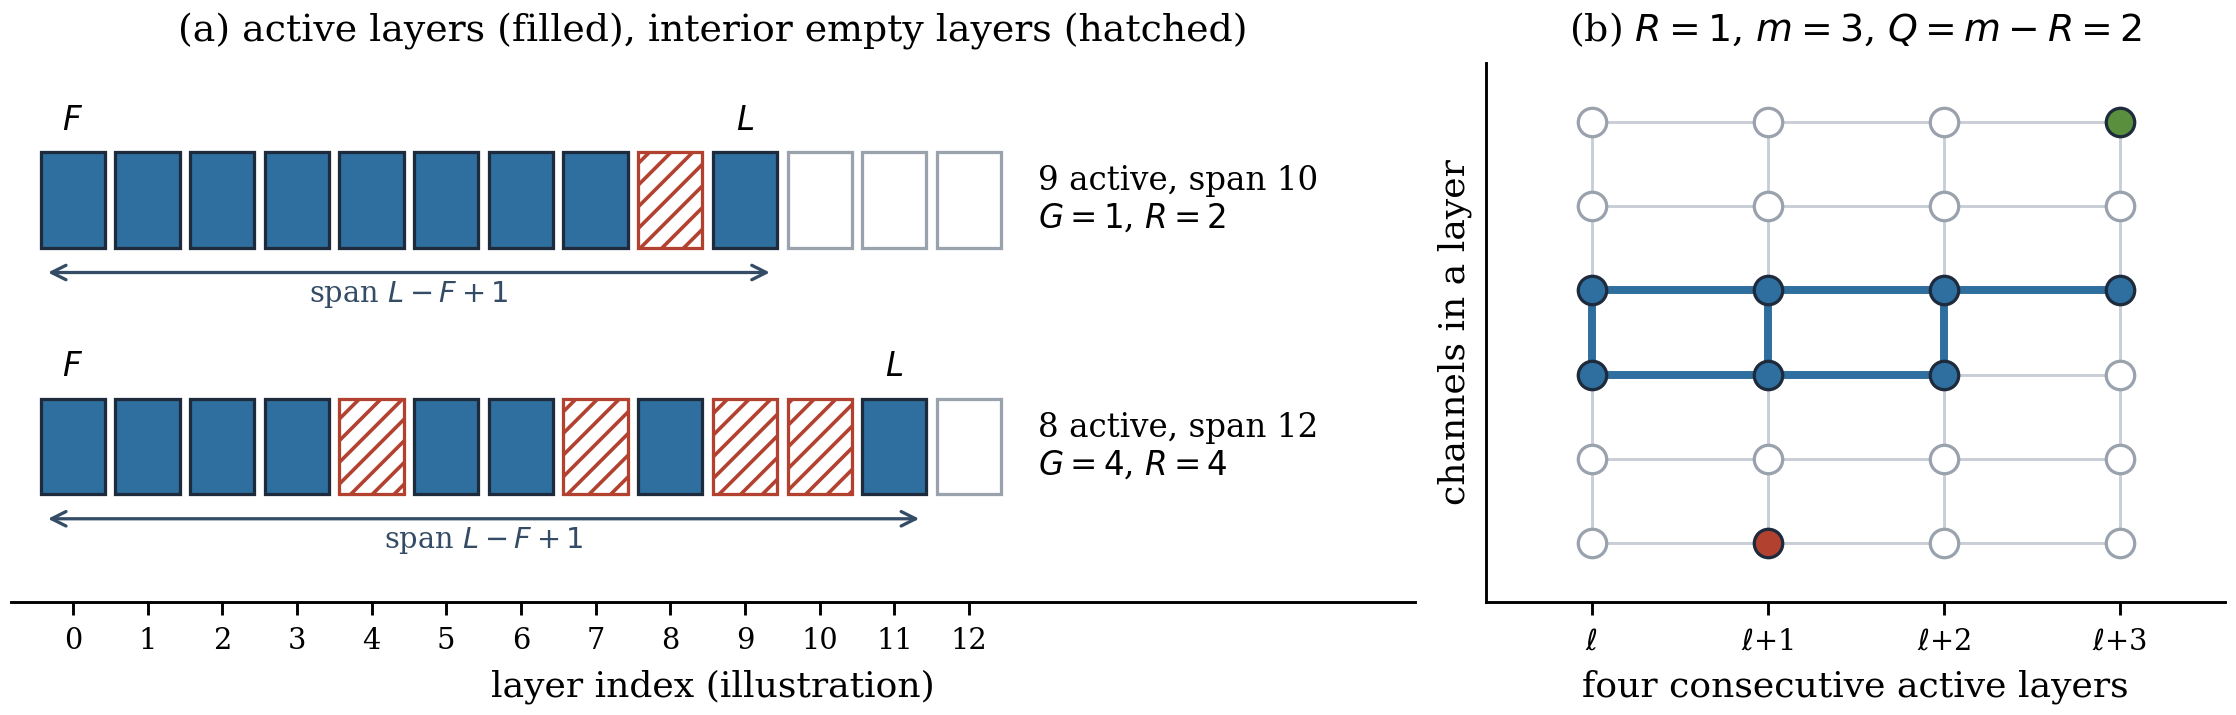
\includegraphics[width=0.98\linewidth]{observable_definitions.png}
 \caption{Definitions of the structural observables (illustration, not data). (a) Two patterns of active layers with first layer $F$, last layer $L$, $G$ empty layers inside the span, and $R$ runs of contiguous active layers. (b) Channels (circles) and graph edges (lines) in four consecutive active layers. The active channels form $m=3$ connected components although the layers form a single run, $R=1$; the excess $Q=m-R=2$ measures fragmentation that empty layers cannot explain.}
 \label{fig:definitions}
\end{figure}

\subsection{Connectivity and a bound from sample means}
\label{sec:bound}

We count the connected components $C_1,\ldots,C_m$ of the readout graph restricted to the active channels $S$ of a shower, ignoring edge direction: two active channels belong to the same component if a path of graph edges through active channels joins them. We also report the fraction of active channels in the largest component, $\max_j|C_j|/|S|$. Components are defined on the graph of Sec.~\ref{sec:data} and are not reconstruction clusters~\cite{atlastopocluster}.

A larger component count can have two origins. Graph edges connect only channels in the same or in adjacent layers, so an empty layer inside the span disconnects everything upstream of it from everything downstream. Let $R$ be the number of runs of contiguous active layers (Fig.~\ref{fig:definitions}). Then $m\geq R$, and we define
\begin{equation}
 Q=m-R\geq0,
 \label{eq:q}
\end{equation}
the number of components in excess of the minimum forced by empty layers. $Q$ counts fragmentation inside runs, as in Fig.~\ref{fig:definitions}(b).

Computing $R$ needs the activity mask of each event, which the evaluation summary does not contain; it contains only the means of $m$ and $G$ and the fraction $f$ of nonempty showers with $G>0$. These suffice for a bound. A shower with $G$ interior empty layers has at most $G+1$ runs, and at least two runs if $G>0$:
\begin{equation}
 1+\mathbf 1_{G>0}\;\leq\;R\;\leq\;G+1 .
 \label{eq:rbound}
\end{equation}
Averaging over a sample (overbars) gives $\overline m-1-\overline G\leq\overline Q\leq\overline m-1-f$. Applying this to each sample and subtracting, with $\Delta$ denoting generated minus Geant4,
\begin{equation}
 \Delta\overline m-\overline G_{\rm gen}+f_{\rm ref}\;\leq\;\Delta\overline Q
 \;\leq\;\Delta\overline m+\overline G_{\rm ref}-f_{\rm gen}.
 \label{eq:qbound}
\end{equation}
Equation~\eqref{eq:qbound} is an exact inequality between sample means. Its width reflects the missing per-event information; it is not a statistical uncertainty.

\subsection{Distances, intervals and the classifier test}

For one-dimensional distributions we use the Wasserstein distance $W_1$, the area between the two empirical cumulative distributions, in the units of the observable~\cite{kansalmetrics}. To give $W_1$ a scale, we also quote the same distance between two disjoint halves of the Geant4 sample (5,000 events each). This half-split value measures finite-sample noise; because each half is smaller than the samples being compared, it is expected to overestimate the noise of the full comparison.

Bootstrap intervals are 95\% percentile intervals from 1,000 resamples of the 10,000 pairs, drawn within each energy bin so that pairing and energy composition are preserved. They exist for the empty-shower fraction, the paired response residual and two Wasserstein distances. For the structural means of Sec.~\ref{sec:results} no interval was computed, so those differences are reported without a statistical uncertainty. All intervals describe resampling of this evaluation sample only; they say nothing about variation between training runs.

A classifier two-sample test (C2ST) trains a classifier to separate generated from Geant4 showers and reports the area under the ROC curve (AUROC) on held-out showers, with 0.5 meaning indistinguishable~\cite{c2st,kansalmetrics}. We use gradient-boosted trees on three sets of inputs: nine shower-shape summaries, the 65 layer energies, and all 6,790 channel energies (Appendix~\ref{app:additional}). The project's screening criterion is an AUROC of at most 0.65 on the shower-shape summaries. Since any classifier gives a lower bound on the separability of two samples, the quoted values are lower bounds.

\section{Results}
\label{sec:results}

Table~\ref{tab:results} summarises the comparison. The mean deposits and the mean numbers of active layers and channels agree at the per-cent level, while the last active layer, the number of interior empty layers and the number of graph components do not.

\begin{table}[H]
\centering
\caption{Generated and Geant4 showers at 10,000 matched incident neutrons. Deposits and empty-shower counts use all events; the structural quantities in the lower block use nonempty showers (9,907 Geant4, 9,858 generated). Differences are generated minus Geant4, computed before rounding; pp denotes percentage points.}
\label{tab:results}
\small
\begin{tabular}{@{}lrrr@{}}
\toprule
Quantity & Geant4 & Generator & Gen. $-$ Geant4 \\
\midrule
Empty showers & 93 (0.93\%) & 142 (1.42\%) & $+49$ ($+0.49$ pp) \\
Mean total deposit (GeV) & 4.324 & 4.369 & $+0.045$ \\
Mean ECAL deposit (GeV) & 2.100 & 2.275 & $+0.175$ \\
Mean HCAL deposit (GeV) & 2.224 & 2.094 & $-0.129$ \\
\midrule
Mean first active layer $F$ & 0.510 & 0.735 & $+0.225$ \\
Mean last active layer $L$ & 56.20 & 60.62 & $+4.42$ \\
Mean number of active layers & 54.58 & 54.83 & $+0.25$ \\
Mean span $L-F+1$ & 56.69 & 60.88 & $+4.20$ \\
Mean interior empty layers $G$ & 2.10 & 6.05 & $+3.95$ \\
Showers with an interior gap & 52.43\% & 93.53\% & $+41.10$ pp \\
Mean number of active channels & 1617.6 & 1588.8 & $-28.7$ \\
Mean number of graph components $m$ & 23.42 & 59.39 & $+35.97$ \\
Mean largest-component fraction & 94.90\% & 88.87\% & $-6.03$ pp \\
\bottomrule
\end{tabular}
\end{table}

\subsection{Deposited energy and empty showers}

The mean total deposit is 4.369\,GeV for generated showers and 4.324\,GeV for Geant4, a difference of 0.045\,GeV or 1.0\%. This difference is not statistically significant. The paired residual $(T_{\rm gen}-T_{\rm ref})/\Kinc$ has a mean of $2.9\times10^{-5}$ with a bootstrap interval of $[-8.5,\,9.3]\times10^{-4}$, which contains zero. Its root-mean-square, 0.046, equals the value expected for two uncorrelated samples with the per-bin standard deviations of Table~\ref{tab:energy_bins} (0.046, taking the energy distribution within each bin as uniform). Sharing the incident condition therefore induces no measurable correlation between the two showers of a pair, and standard errors can be computed as for independent samples. For the difference of the mean total deposits the standard error is 0.068\,GeV, so the observed difference is 0.7 standard errors. The distribution of $T$ also agrees within sampling noise, with $W_1=0.073$\,GeV against half-split values of 0.135 and 0.147\,GeV.

The agreement of the total hides opposite shifts in the two sections. The generated ECAL deposit is higher by 0.175\,GeV (8.3\%) and the HCAL deposit lower by 0.129\,GeV (5.8\%); in the generator this split is set by the layer-energy flow of Eq.~\eqref{eq:layer_budget}. Figure~\ref{fig:longitudinal} shows where the HCAL deficit sits: the generated mean profile is low by 8.6\% at the Geant4 maximum in layer 9 and by up to 12\% in layers 10--16. The shift between sections is not a sampling fluctuation: the distribution of the ECAL energy fraction differs by 9.5 times the half-split scale (Table~\ref{tab:distances}). Because the two sections would enter a calibrated energy with different weights, the cancellation in the unweighted sum should not be expected to survive calibration.

\begin{figure}[!htbp]
 \centering
 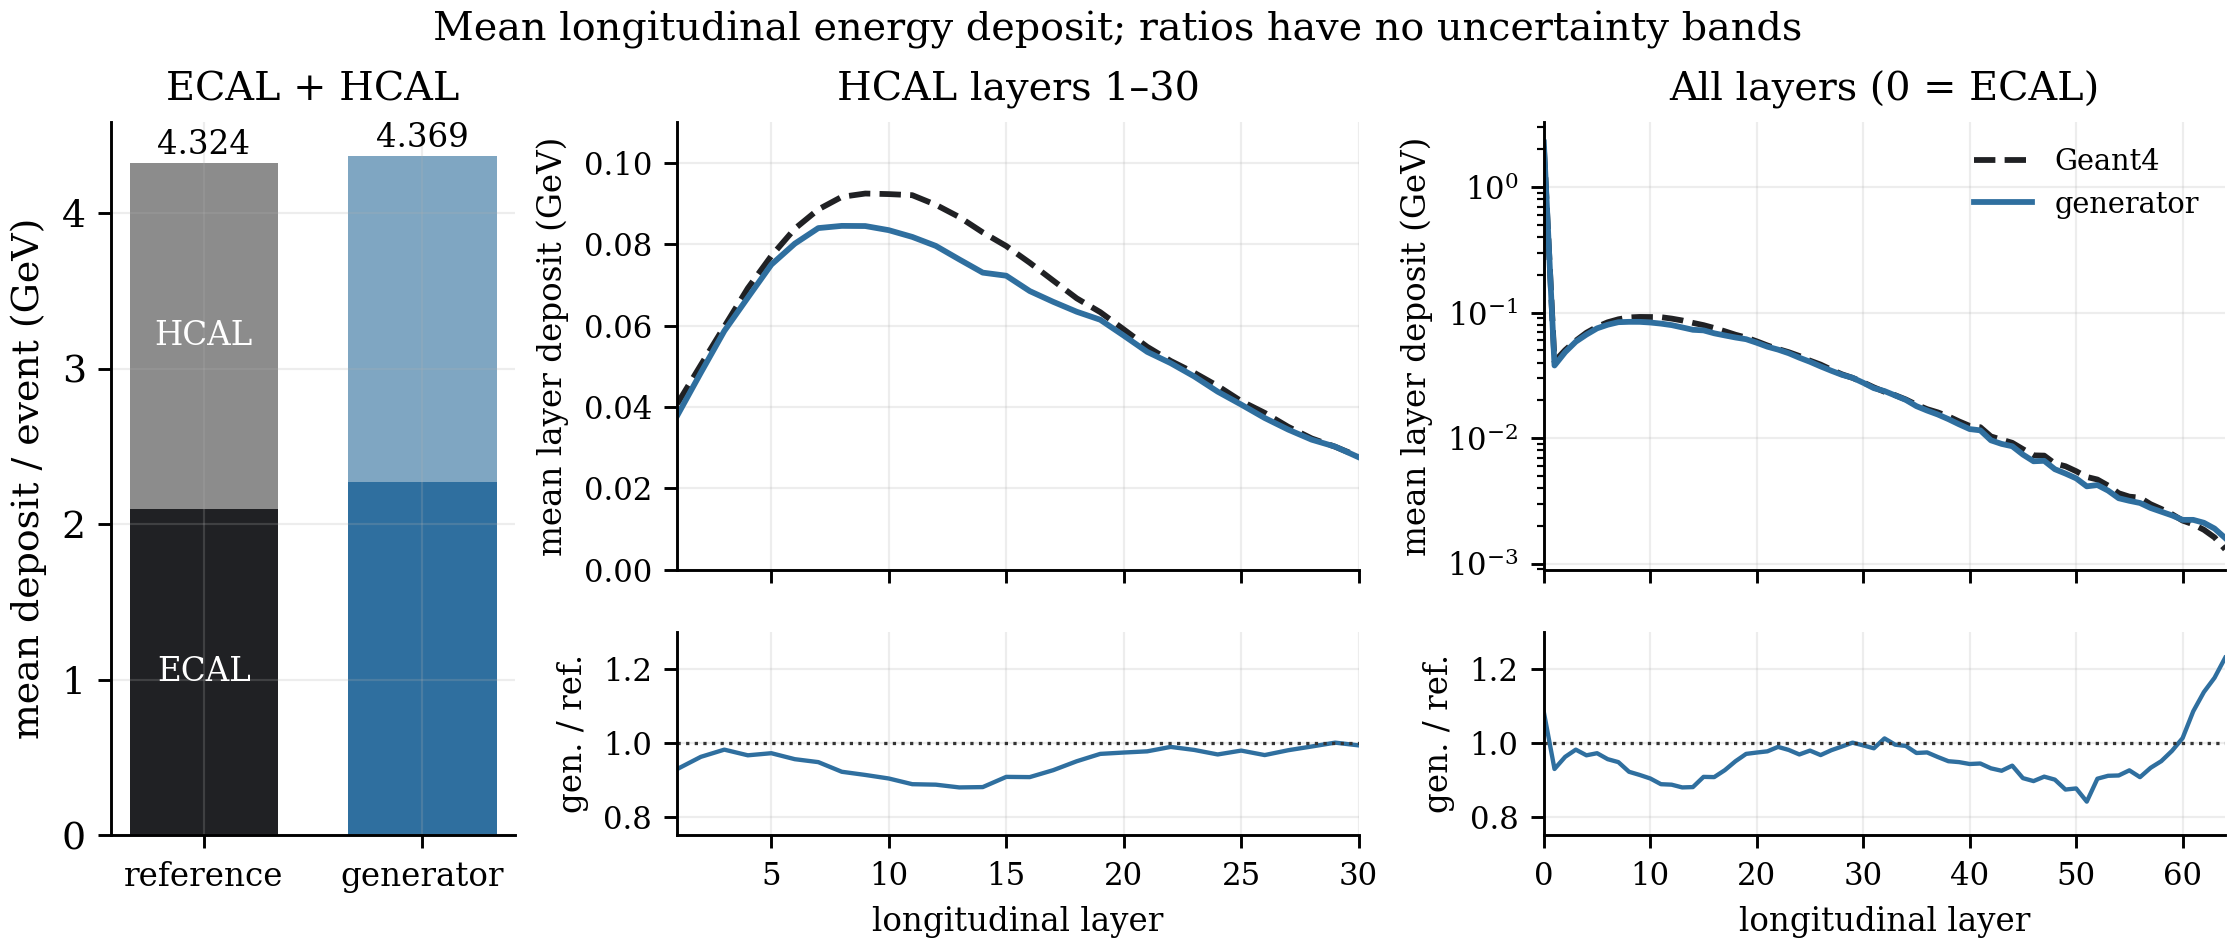
\includegraphics[width=\linewidth]{longitudinal_profile.png}
 \caption{Mean deposited energy per event over all 10,000 events, including empty showers. Left: ECAL and HCAL contributions to the mean total; the generator is high in the ECAL and low in the HCAL. Centre: HCAL layers 1--30 on a linear scale. Right: all layers on a logarithmic scale, with the ECAL as layer 0. Dashed curves are Geant4, solid curves the generator; the lower panels show the ratio of the two means. No uncertainty band is available for the profiles.}
 \label{fig:longitudinal}
\end{figure}

In bins of incident energy (Table~\ref{tab:energy_bins} in Appendix~\ref{app:additional}), the relative difference of the mean deposit ranges from $-7.7\%$ to $+7.7\%$ with alternating sign. With about 1,250 events per bin and a spread of $T$ as large as its mean, the standard error of the difference of the two bin means is 4--5\% of the mean. The binned differences are at most 2.0 standard errors, with $\chi^2=13.0$ for eight bins, and do not establish an energy-dependent bias.

The generator produces 142 empty showers against 93 in Geant4. The difference of 0.49 percentage points has a bootstrap interval of 0.19--0.76 percentage points and is therefore resolved: the generator produces empty showers about 1.5 times as often as Geant4. The evaluation summary does not record $V_0$, so the 142 cannot be divided between the hurdle and the clipping at zero in Eq.~\eqref{eq:cap}.

\subsection{Longitudinal activity}

Generated showers have almost the same mean number of active layers as Geant4 showers (54.83 against 54.58), but those layers are spread over a longer range. The mean first active layer moves by $+0.225$ and the mean last active layer by $+4.42$; 92.53\% of generated nonempty showers start in the ECAL, against 93.81\% for Geant4. The span therefore grows by 4.20 layers while the number of active layers grows by 0.25, and the difference, 3.95 layers, is the increase in interior empty layers $G$ from 2.10 to 6.05. The fraction of nonempty showers with at least one interior gap rises from 52.43\% to 93.53\%.

The additional depth carries little energy. The energy-weighted mean depth, $\sum_\ell\ell B_\ell/T$, averaged over nonempty showers, is 14.14 layers for the generator and 14.15 for Geant4. The mean energy deposited in layers 57--64, the region into which the mean last active layer moves, is 17.8\,MeV per event for the generator and 17.2\,MeV for Geant4, 0.4\% of the total in both cases. The mean profiles of Fig.~\ref{fig:longitudinal} agree within 25\% in every layer. The discrepancy is thus one of occupancy pattern: which layers record any deposit at all, rather than how much energy they record on average. Mean depth is nevertheless not matched event by event; the distribution of the energy-weighted depth differs by $W_1=0.97$ layers, six times the half-split value (Table~\ref{tab:distances}).

\subsection{Channel support and graph connectivity}

Generated showers have on average 28.7 fewer active channels than Geant4 showers ($-1.8\%$) but 35.97 more graph components, 59.39 against 23.42. The largest component contains 88.87\% of the active channels on average, against 94.90\% for Geant4. Geant4 showers are thus already fragmented on this graph when every positive deposit counts, with about 22 small components besides the main one; the generator produces roughly two and a half times as many.

Inserting the means of Table~\ref{tab:results} into the bounds of Sec.~\ref{sec:bound} gives $20.32\leq\overline Q_{\rm ref}\leq21.89$ and $52.34\leq\overline Q_{\rm gen}\leq57.45$, and from Eq.~\eqref{eq:qbound}
\begin{equation}
 30.45\;\leq\;\Delta\overline Q\;\leq\;37.14 ,
 \label{eq:qresult}
\end{equation}
shown in Fig.~\ref{fig:support}. Equivalently, the mean number of runs differs by between $-1.17$ and $+5.52$. Of the 35.97 additional components, at most 5.52 (15.4\%) can be the direct consequence of additional empty layers; at least 30.45 (84.6\%) are additional components within runs of contiguous active layers. The fragmentation excess is therefore not simply the splitting of showers by additional empty layers. Whether the two discrepancies share a cause further upstream in the generator is a separate question (Sec.~\ref{sec:interpretation}).

\begin{figure}[!htbp]
 \centering
 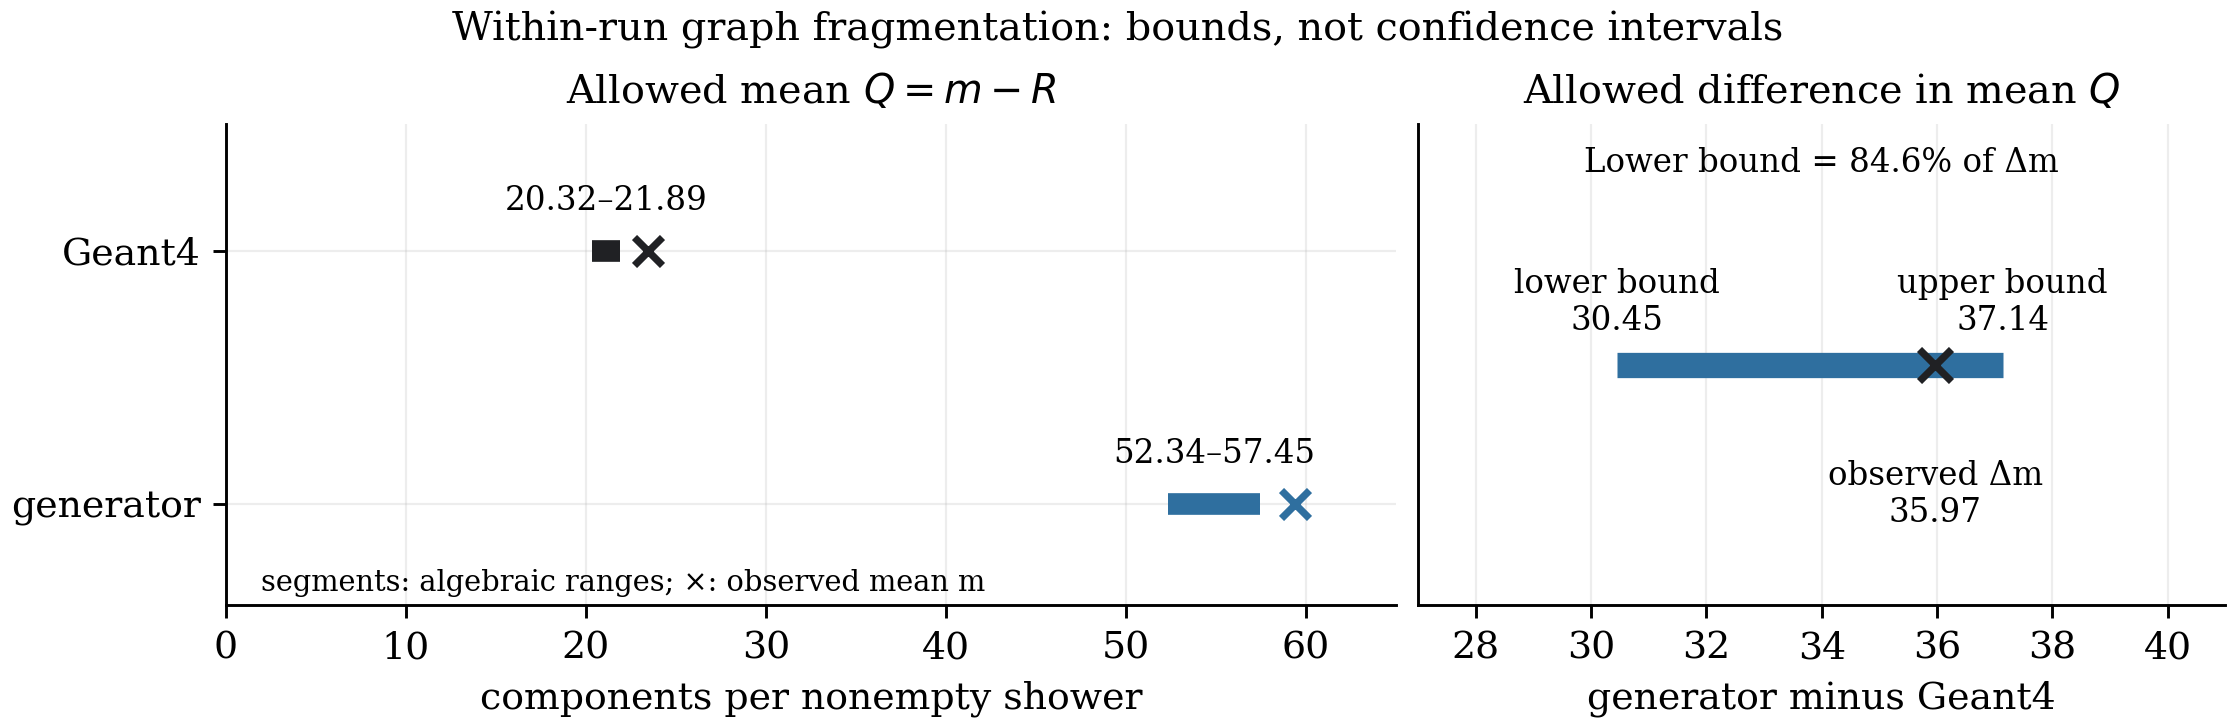
\includegraphics[width=\linewidth]{support_summary.png}
 \caption{Graph fragmentation in nonempty showers. Left: the measured mean number of components $m$ (crosses) and the range allowed for the mean within-run excess $\overline Q=\overline m-\overline R$ by Eq.~\eqref{eq:rbound} (bars). Right: the range allowed for the difference $\Delta\overline Q$ by Eq.~\eqref{eq:qbound}, compared with the measured difference $\Delta\overline m$. The bars are exact algebraic bounds that follow from the sample means; they are not statistical uncertainties.}
 \label{fig:support}
\end{figure}

A within-run component need not be a lateral effect: active channels in adjacent active layers can also fail to be linked by the four-neighbour longitudinal edges. The bound does not distinguish the two cases.

Two further numbers describe the channel pattern. The distribution of the number of active channels, over all events, differs by $W_1=58.68$ channels (bootstrap interval 51.47--66.92), about four times the half-split values of 13.78 and 15.82. The fraction of graph edges with both ends active is 0.1375 for the generator and 0.1458 for Geant4; this measure is not corrected for the difference in occupancy and is quoted for completeness.

\subsection{Shower-shape distributions}

Table~\ref{tab:distances} extends the comparison to the nine event-level summaries used by the classifier, each compared through its full distribution. The total deposit and the transverse centroid agree within the half-split scale. The remaining six summaries differ by four to ten times that scale. Generated showers put a larger fraction of their energy in the ECAL (0.263 against 0.235 on average), are narrower by about 3\% in transverse RMS, and concentrate more energy in their highest-energy channel. In terms of the stages of Table~\ref{tab:stages}, the first of these is a property of the layer-energy flow, and the other two of the channel selection and the channel-energy flow.

\begin{table}[!htbp]
\centering
\caption{Event-level shower summaries over all 10,000 events. $W_1$ is the Wasserstein distance between the generated and Geant4 distributions; the half-split column is the same distance between two halves of the Geant4 sample and sets the scale of sampling noise. Fractions are relative to the event total $T$; an empty shower enters every summary as zero. Positions are in the coordinate frame of Fig.~\ref{fig:geometry}. No interval is available for the ratios.}
\label{tab:distances}
\small
\begin{tabular}{@{}lrrrrr@{}}
\toprule
Summary & Geant4 mean & Generator mean & $W_1$ & Half-split $W_1$ & Ratio \\
\midrule
Total deposit $T$ (GeV) & 4.324 & 4.369 & 0.073 & 0.135 & 0.5 \\
Centroid $x$ (mm) & $-906.8$ & $-902.8$ & 4.50 & 5.69 & 0.8 \\
Centroid $y$ (mm) & $-33.2$ & $-31.9$ & 1.71 & 2.15 & 0.8 \\
\midrule
Active channels & 1602.5 & 1566.3 & 58.7 & 15.8 & 3.7 \\
Energy-weighted depth (layers) & 14.02 & 13.94 & 0.971 & 0.155 & 6.3 \\
Largest-channel fraction & 0.1549 & 0.1659 & 0.0130 & 0.0021 & 6.3 \\
Fraction in layers 48--64 & 0.0221 & 0.0252 & 0.0083 & 0.0013 & 6.5 \\
Transverse RMS (mm) & 86.34 & 83.48 & 3.34 & 0.49 & 6.9 \\
ECAL fraction & 0.2354 & 0.2626 & 0.0280 & 0.0029 & 9.5 \\
\bottomrule
\end{tabular}
\end{table}

Correlations between layers are also not reproduced at the level of sampling noise: the Frobenius distance between the generated and Geant4 $65\times65$ correlation matrices of the layer energies is 3.52, against 1.98 between the two Geant4 halves.

\subsection{Classifier test}

On the 10,000 pairs, the classifier reaches a mean AUROC over three classifier seeds of 0.775 on the shower-shape summaries, 0.791 on the channel energies and 0.856 on the layer energies (Table~\ref{tab:classifier_seeds}). The first value exceeds the screening criterion of 0.65: the generated showers are readily distinguishable from Geant4.

Two features of these numbers need comment. First, the train/test split of this evaluation was made by shower and not by pair, so the two members of a pair, which share $\Kinc$ exactly, can fall on opposite sides of the split. A control classifier given only $\Kinc$ then scores 0.464, below 0.5, because it learns the label of a training shower and meets its partner, with the opposite label, in the test set. The control shows that this split biases the test; for inputs correlated with $\Kinc$ the bias is towards lower AUROC. A separate evaluation of the same checkpoint that keeps pairs together, on a different sample of 8,000 showers, gives 0.500 for the control and 0.893 for the shower-shape summaries. The two evaluations use different events and cannot be combined. Both lie well above the criterion; the pair-grouped one has the sounder design and the larger value. Second, the classifier given all channel energies does worse than the one given only the 65 layer sums, which are linear combinations of the channel energies. A classifier of this size evidently does not exploit the channel-level information, so the channel-level value in particular should be read as a loose lower bound.

\subsection{Numerical consistency}

All 10,000 generated showers satisfy the identities of Sec.~\ref{sec:model} to single-precision accuracy: no deposit is negative or non-finite, every layer has exactly the requested number of active channels, and the largest absolute differences between summed channel energies and the sampled layer and event energies are $3.05\times10^{-5}$ and $1.14\times10^{-5}$\,GeV. No selected channel received a deposit that rounded to zero, which would have changed the support observables. These checks concern internal consistency only.

\FloatBarrier
\section{Discussion}
\label{sec:discussion}

\subsection{Interpretation and a candidate mechanism}
\label{sec:interpretation}

The generator reproduces the mean energy and mean occupancy of Geant4 showers while distributing its active layers and channels differently: active layers that reach further downstream with more empty layers between them, and more disconnected groups of channels. Since the additional depth carries well under 1\% of the energy, the discrepancy lives in the low-energy periphery of the shower. That does not make it harmless, because hit-based reconstruction and any threshold act on individual channels; whether it matters is a question for a threshold scan and a reconstruction study, not for the mean profile.

For the gap excess, the model contains a direct candidate cause. Equation~\eqref{eq:activity} switches each layer after the first on or off independently, given $(h_c,T,F)$. Independence preserves the mean number of active layers but not their contiguity. A three-layer example makes this concrete. Fix $F=0$ and suppose that in the reference layers 1 and 2 are either both active, with probability $p$, or both inactive. Independent draws with the same per-layer probability $p$ leave the mean number of active layers unchanged at $1+2p$, but produce the pattern (active, empty, active) with probability $p(1-p)$, which never occurs in the reference, and raise the mean last active layer by $p(1-p)$. This is the signature in Table~\ref{tab:results}: an unchanged number of active layers, a deeper last layer, and more interior gaps. The example shows that the factorisation can produce the effect, not that it accounts for its size; layers remain correlated through the sampled $T$ and $F$, and Geant4 showers themselves have interior gaps in 52\% of cases.

Two measurements would settle the question. The first samples activity masks from the per-layer Geant4 activity probabilities in narrow bins of energy, direction, $T$ and $F$, independently per layer: if this reproduces the generated gap and last-layer shifts, the factorisation is sufficient to explain them. The second replaces the generated mask by the Geant4 mask and runs the later stages unchanged: if the gap excess disappears but the fragmentation excess remains, the two discrepancies have separate origins. Models that treat the dependence between layers explicitly, such as L2LFlows and iCaloFlow~\cite{l2lflows,icaloflow}, are the natural comparison for a replacement of the activity stage.

For the fragmentation within runs, the candidates are the count stage and the selection stage. The scores of Eq.~\eqref{eq:message} see the neighbourhood of each channel, but the Gumbel perturbations of Eq.~\eqref{eq:topk} are independent, and a score trained with a per-channel cross entropy is not guaranteed to give the correct inclusion probability once exactly $K_\ell$ channels are drawn. Comparing the generated and Geant4 occupancy of each channel at fixed layer and count, and drawing channels from the Geant4 per-channel occupancies without any neighbour correlation, would show how much of the fragmentation is explained by miscalibrated or uncorrelated selection. The energy flow cannot repair the support, as noted in Sec.~\ref{sec:model}.

\subsection{Limitations}
\label{sec:limitations}

\begin{description}[leftmargin=1.2em,itemsep=3pt]
 \item[No readout threshold.] An active channel is any channel with a positive Geant4 deposit. The mean deposit per active channel is 2.7\,MeV for Geant4 and 2.8\,MeV for the generator, but the spectrum is not available, and the structural observables may be dominated by deposits far below any realistic threshold. The design study uses a MIP scale of 0.5\,MeV, keeps hits above 0.5\,MIP, and requires $t<275$\,ns~\cite{epiczdc}. Repeating Table~\ref{tab:results} as a function of a channel threshold, beginning near 0.25\,MeV in the HCAL, is the most important missing measurement. A time cut cannot be applied consistently, since the generator has no hit times.
 \item[Means only.] For the structural observables only sample means are available. Their distributions, their dependence on energy, the exact run counts, the size and energy of the components, and statistical intervals all require per-event information.
 \item[One training run.] There is one checkpoint from one random seed, trained on 4.35\% of the training partition and selected on a noisy validation curve (Fig.~\ref{fig:training}). The results cannot separate properties of the architecture from those of this particular fit. At least three seeds and a fit to the full training partition are needed.
 \item[Evaluation sample.] The 10,000 events were reused during development, and each condition was generated once, so the spread of generated showers at a fixed condition was not examined. The generated and Geant4 nonempty subsets are selected separately and differ in size by 49 events.
 \item[Detector description.] The geometry tag, materials, Geant4 configuration and identifier map of the sample are not documented (Sec.~\ref{sec:data}). The graph is built from channel centroids and was also used by the generator; an independently defined physical-neighbour graph could give different component counts for both samples.
 \item[Conditioning.] The condition has no impact position. If neutrons of the same direction strike the detector at different points, the model cannot learn the dependence of containment and acceptance on position, which may contribute to the excess of empty showers. Acceptance is likely to matter: the Geant4 empty fraction of 0.93\% is about ten times the probability, $e^{-7}\approx0.1\%$, that a neutron crosses seven interaction lengths without interacting.
 \item[Unstudied settings.] The number of flow steps, the selection temperature $\tau$, the loss weights and the response cap were not varied.
\end{description}

\subsection{Computing cost}

Generation time was not measured in isolation. The complete evaluation of the 10,000 pairs, including generation, took 3,442\,s on one GPU in single precision at a batch size of eight. Of this, 1,009\,s were spent in timed analysis steps (connected components, classifiers and bootstrap), which leaves at most 0.24\,s per shower for generation together with data loading and consistency checks. This is an upper limit under untuned conditions, not a benchmark, and no Geant4 time per event is available for the sample; a speed-up therefore cannot be quoted.

\section{Conclusion}

For a hierarchical flow-matching generator of neutron showers in an ePIC zero-degree calorimeter simulation, agreement with Geant4 in mean deposited energy (1.0\%) and in the mean number of active layers (0.25 layers) coexists with clear disagreement in spatial structure. The last active layer is 4.42 layers deeper, there are 3.95 more empty layers inside the occupied range, and the number of connected components on the readout graph is 59.39 instead of 23.42. A bound derived from sample means shows that at least 30.45 of the 35.97 additional components arise within contiguous active layers, so the fragmentation is not simply the splitting of showers by the additional empty layers. Shower-shape distributions and a classifier test confirm that the two samples are distinguishable.

The practical lesson for validating calorimeter surrogates is that mean response and mean occupancy should be accompanied by observables that are sensitive to the contiguity of the shower, such as interior gaps and graph components; these are inexpensive and exposed here a discrepancy that the means do not show. For this model, the factorised layer-activity stage is the leading candidate cause of the gap excess. The decisive next measurements are the dependence of all structural observables on a channel threshold, their per-event distributions, and the activity tests of Sec.~\ref{sec:interpretation}.

\section*{Code and data availability}

The \href{https://github.com/JulianAttemptsCoding/fast-mc-paper}{project repository} contains the evaluation summary, the channel geometry, the training history, the figure scripts and the manuscript source. The simulated events and the model checkpoint belong to the collaboration and are not redistributed; generation, retraining and per-event studies require them.

\section*{Acknowledgments}

The author thanks Dr. Wen-Chen Chang (Institute of Physics, Academia Sinica) for his generous mentorship, guidance, and encouragement, and the Institute of Physics laboratory community for their welcome and support.

\section*{Author contributions and use of generative AI}

Julian Juan: conceptualization, methodology, software, investigation, visualization, and writing.

OpenAI Codex assisted with software and manuscript drafting, specification review, literature searches, and editing. The author supplied the research ideas, checked the work, and takes responsibility for the scientific content.

\appendix
\section{Settings and reproducibility}
\label{app:reproducibility}

\paragraph{Checkpoint.} The analysed checkpoint is epoch 90 of run \texttt{dicos-f-02} in the \texttt{calibrated\_lr3e4} series, training seed 20260723, validation objective 4.4837676194. Its SHA-256 is
\begin{quote}\footnotesize\nolinkurl{491284c7423f365230d34b0443f95aa4888ec770bdc673c4c979897bad8acbce}\end{quote}
and that of its configuration file is
\begin{quote}\footnotesize\nolinkurl{116bc8c220b07ce54ae07196bdd6ed8e835775c8c937182a209a799dc94ae9c5}\end{quote}
The available training history covers epochs 11--114 of joint training (Fig.~\ref{fig:training}). The durations of the single-stage phases, the remaining optimiser settings and the software environment are not part of the paper repository. Training ran on a single NVIDIA RTX~4090 (24\,GB) at about 13 minutes per epoch.

\paragraph{Loss weights.} Table~\ref{tab:weights} lists the weights of Eq.~\eqref{eq:joint_loss}. They were obtained by measuring, on training batches, the median gradient norm of each loss term with respect to the condition encoder, taking the inverse of each median relative to their geometric mean, clipping to $[0.25,4]$, and rescaling the nine weights to a mean of one. The rescaling is why entries of the table lie outside the clipping interval. The weights of the total-deposit, layer-energy and count terms sit at the lower clipping bound and the visibility weight at the upper one. The table reproduces the calibration record; the configuration file actually used in training was not available for an independent check.

\begin{table}[H]
\centering
\caption{Loss weights of Eq.~\eqref{eq:joint_loss}, rounded to six decimals.}
\label{tab:weights}
\small
\begin{tabular}{@{}clr@{}}
\toprule
Weight & Term & Value \\
\midrule
$w_{V}$ & Visibility & 2.574417 \\
$w_{T}$ & Total deposit & 0.160901 \\
$w_{F}$ & First active layer & 2.159451 \\
$w_{A}$ & Layer activity & 0.536770 \\
$w_{B}$ & Layer-energy flow & 0.160901 \\
$w_{K}$ & Channel count & 0.160901 \\
$w_{S}$ & Channel selection, BCE & 1.324108 \\
$w_{R}$ & Channel selection, ranking & 1.477591 \\
$w_{Y}$ & Channel-energy flow & 0.444960 \\
\bottomrule
\end{tabular}
\end{table}

\paragraph{Evaluation run.} The generated sample was drawn with seed 20260723 (the same integer as the training seed, used independently), in single precision on a GPU, in batches of eight, with eight steps for each flow. The list of evaluation events has SHA-256
\begin{quote}\footnotesize\nolinkurl{1bc3a6b21f736fc71551580a93207128c043833c6848627fb16f07475931690a}\end{quote}
The consistency checks of Sec.~\ref{sec:results} used a tolerance, per batch, of the larger of $2\times10^{-5}$\,GeV and $10^{-5}$ times the largest event total in the batch. The largest layer residual, $3.05\times10^{-5}$\,GeV, exceeds the absolute part of this tolerance and passes through the relative part.

\paragraph{Data partitions.} The split is by a hash of the event identifier, not by simulation job. This study uses validation events only. Earlier work in the same project inspected 40,000 events of the test partition in a classifier study and a further sample containing 200 test events; these did not inform any model decision, but the test partition is not untouched. Between 36,100 and 36,300 test events have not been inspected, and their identities would have to be established before they are used as a blind sample.

\section{Energy bins and classifier details}
\label{app:additional}

\begin{table}[H]
\centering
\caption{Total deposit in bins of incident kinetic energy, over all events including empty showers. $n$ is the number of pairs; $\mu$ and $\sigma$ are the mean and (population) standard deviation of $T$ in GeV. The differences are $100(\mu_{\rm gen}/\mu_{\rm ref}-1)$ and $100(\sigma_{\rm gen}/\sigma_{\rm ref}-1)$. Bins include their lower edge; the last bin also includes 250\,GeV. Combining the bins gives standard deviations of 4.759 and 4.830\,GeV for the full Geant4 and generated samples.}
\label{tab:energy_bins}
\small
\begin{tabular}{@{}rrrrrrrr@{}}
\toprule
$\Kinc$ (GeV) & $n$ & $\mu_{\rm ref}$ & $\mu_{\rm gen}$ & Mean diff. (\%) & Width diff. (\%) & $\sigma_{\rm ref}$ & $\sigma_{\rm gen}$ \\
\midrule
50--75 & 1,182 & 2.398 & 2.216 & $-7.59$ & $-6.40$ & 2.830 & 2.649 \\
75--100 & 1,270 & 2.892 & 2.908 & $+0.57$ & $+2.80$ & 3.154 & 3.243 \\
100--125 & 1,310 & 3.527 & 3.513 & $-0.42$ & $-0.72$ & 3.872 & 3.845 \\
125--150 & 1,226 & 3.849 & 4.146 & $+7.74$ & $+9.58$ & 3.921 & 4.297 \\
150--175 & 1,288 & 4.867 & 4.494 & $-7.65$ & $-10.89$ & 5.037 & 4.488 \\
175--200 & 1,268 & 5.030 & 5.320 & $+5.76$ & $+8.79$ & 4.802 & 5.224 \\
200--225 & 1,266 & 5.921 & 6.026 & $+1.78$ & $-1.70$ & 6.127 & 6.023 \\
225--250 & 1,190 & 6.095 & 6.330 & $+3.85$ & $+5.24$ & 5.827 & 6.133 \\
\bottomrule
\end{tabular}
\end{table}

\begin{table}[H]
\centering
\caption{Classifier AUROC on the 10,000 pairs for three classifier seeds. The seeds change the classifier and its train/test split; the generator is the same in all columns.}
\label{tab:classifier_seeds}
\small
\begin{tabular}{@{}lrrrr@{}}
\toprule
Inputs & 20260804 & 20260805 & 20260806 & Mean \\
\midrule
$\Kinc$ only (control) & 0.4739 & 0.4624 & 0.4545 & 0.4636 \\
Shower-shape summaries & 0.7789 & 0.7719 & 0.7735 & 0.7748 \\
Channel energies & 0.7873 & 0.7943 & 0.7914 & 0.7910 \\
Layer energies & 0.8490 & 0.8580 & 0.8623 & 0.8564 \\
\bottomrule
\end{tabular}
\end{table}

\paragraph{Classifier.} The classifier is a histogram gradient-boosting model with at most 100 boosting iterations, maximum depth four and learning rate 0.08; other options are library defaults. A random split, stratified by class, assigns 14,000 of the 20,000 showers to training and 6,000 to testing, and the same seed controls the split and the classifier. Because the split does not keep pairs together, 42\% of pairs are divided between the two sets in expectation, and a test shower has a 70\% chance that its partner is in the training set.

\paragraph{Inputs.} The nine shower-shape summaries are those of Table~\ref{tab:distances}: total deposit, number of active channels, energy-weighted depth, energy-weighted centroid in $x$ and $y$, energy-weighted transverse RMS about that centroid, fraction of the energy in the highest-energy channel, fraction in the ECAL, and fraction in layers 48--64. Quantities divided by the total use a floor of $10^{-9}\GeV$ in the denominator. The other input sets are the 65 layer energies, the 6,790 channel energies, and $\Kinc$ alone. These settings were read from an archived copy of the evaluation code; the library version used at the time was not recorded.

\Needspace{8\baselineskip}
\printbibliography

\end{document}
